\textbf{{因特网有两大路由选择协议:}}

\textbf{1.内部网关协议(IGP)}

内部网关协议是\textbf{在一个自治系统内部使用的路由选择协议},它与互联网中其他自治系统选用什么路由选择协议无关。目前这类路由选择协议使用得最多,如RIP和OSPF路由协议。

\textbf{2.外部网关协议(EGP)}

若源站和目的站处在不同的自治系统中,当数据报传到另一个自治系统的边界时\textbf{(这两个自治系统可能使用不同的内部网关协议),就需要使用一种协议将路由选择信息传递到另一个自治系统中},如下图所示。这样的协议就是外部网关协议,如BGP-4。

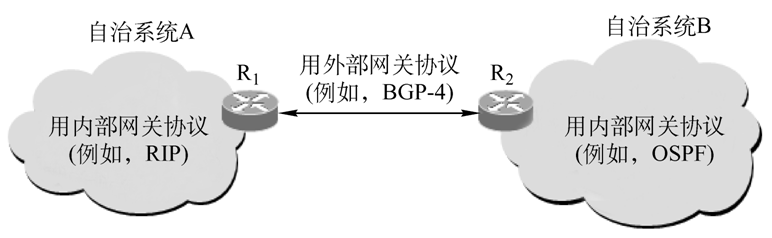
\includegraphics[width=3.12500in,height=0.95833in]{png-jpeg-pics/29BAEA565A731F32C14A2358F2264E1A.png}
